\documentclass[fleqn]{jbook}
\usepackage{physpub}

\begin{document}

\begin{question}{専攻 問題5}{}


図1 のように質量がそれぞれ、 $m, M (m < M)$ である2種の原子を交互に
配置した鎖状の 1次元格子の振動を考える。ポテンシャルは各最近接原子間
のみに働き、微小な平衡位置からのずれに対して調和型であり、原子は鎖の
方向にだけ変位すると仮定する。以下の設問に答えよ。

\begin{subquestions}
\SubQuestion
  原子間のポテンシャルのばね定数を k 、 $n$ 番目の単位胞内の質量$m$
  の原子の変位を $x_n$ 、 質量 $M$ の原子の変位を $y_n$ とするとき、
  それらの運動方程式はどのようになるか?


\SubQuestion
  この系の基準振動は一般に、
%
  \begin{eqnarray*}
    x_n &=& A \exp ( - i\omega t) \exp (i n q a) \\
    y_n &=& B \exp ( - i\omega t) \exp (i n q a)
  \end{eqnarray*}
%
  と表すことができる。ここで、 $t$ は時間、 $\omega$ は角振動数、
  $q$ は波数、 $a$ は原子間の距離の 2 倍である。 $A$ と $B$ の
  満たす関係式を導け。


\SubQuestion
  $\omega$ は $q$ のどの様な関数になるか? またその関係 $\omega (q)$ 
  を図で示せ。図には波数 $q$ が 0 , および $\pi/a$ のときの$\omega$
  の値を記入すること。


\SubQuestion
  $q=\pi/a$ のときの基準振動に対応する各原子の変位を図示し、このとき
  の振動数 $\omega$ がなぜそのような値をとるかについて考察せよ。


\SubQuestion
  $m$ が $M$ に比べて極めて小さいとき、この格子系の振動はどのような
  特徴を示すか考察せよ。またそのような特徴がなぜ出現するかについて、
  理由を考えてみよ。

\end{subquestions}

\begin{center}
  \mbox{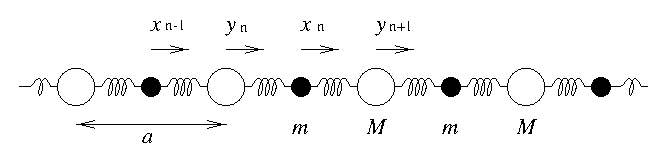
\includegraphics[clip]{1994phy5-1.eps}}
\end{center}

\end{question}
\begin{answer}{専攻 問題5}{}

\begin{subanswers}
\SubAnswer
  原子の運動方程式は以下の通り。
%
  \begin{eqnarray}
    m \Deriver{^2}{t^2} x_n &=& -k (x_n - y_n) + k(y_{n+1} - x_n) \nonumber \\
    M \Deriver{^2}{t^2} y_n &=& -k (y_n - x_{n-1}) + k(x_n - y_n) \eqname{1}
  \end{eqnarray}
%

\SubAnswer
  与えられた $x_n,y_n$ の表式を前問の運動方程式に代入して整理して
%
  \begin{eqnarray}
    (2k - m\omega^2) A - k(1 + e^{+iqa}) B &=& 0 \nonumber \\
    (2k - M\omega^2) B - k(1 + e^{-iqa}) A &=& 0 \eqname{2}
  \end{eqnarray}
%
  を得る。

\SubAnswer
  $A$、$B$ が $A=B=0$ 以外の解をもつためには前問より、
%
  \[ \left|\begin{array}{cc}
       2k-m\omega^2   & -k(1+e^{+iqa}) \\
       -k(1+e^{-iqa}) & 2k-M\omega^2
     \end{array}\right| = 0 \]
%
  であることがわかる。これを $\omega$ について解いて
%
  \begin{equation}
    \omega^2 = \frac{k(m+M)%
              \pm k \sqrt{(m+M)^2-4mM \sin^2{(qa/2)}}}{mM}
    \eqname{3}
  \end{equation}
%
  を得る。分散関係は下図のようになる。

  \begin{center}
    \mbox{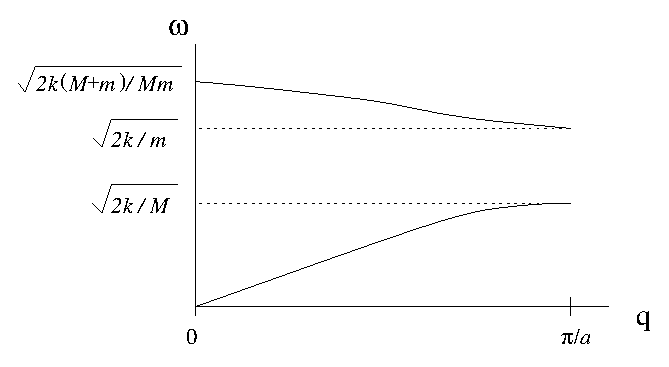
\includegraphics[clip]{1994phy5-2.eps}}
  \end{center}



\SubAnswer
  $q=\pi/a$ を式\eqhref{3}に代入して
%
  \[ \omega^2 = \frac{2k}{M} \quad {\rm or} \quad \frac{2k}{m} \]
%
  を得る。この$\omega$をそれぞれ式\eqhref{2}に代入すると $A,B$の
  条件は、
%
  \[ (a) \quad \omega^2 = \frac{2k}{M} \longrightarrow%
         A = 0 \quad B = 任意 \]
  \[ (b) \quad \omega^2 = \frac{2k}{m} \longrightarrow%
         A = 任意 \quad B = 0 \]
%
  となる。よって、 $q = \pi/a$ の基準振動での各原子の変位は下図の
  ようになる。
%
  \begin{center}
    \mbox{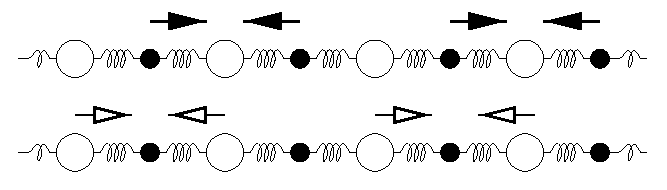
\includegraphics[clip]{1994phy5-3.eps}}
  \end{center}
%
  つまり、それぞれ片方の種類の原子が静止しているため、バネ定数 $2k$
  で原子をつなげていることになっている。


\SubAnswer
  両原子の振幅の比の絶対値を考える。式\eqhref{2}より
%
  \[ \Bigl|\frac{A}{B}\Bigr|=\frac{|2k-M\omega^2|}{|k(1+e^{-iqa})|} \]
%
  これに式\eqhref{3}の$\omega$を代入して $m\ll M$を用いて近似計算
  していく。
%
  \begin{eqnarray*}
    \Bigl|\frac{A}{B}\Bigr|%
      &=& \frac{\bigl|2m-(m+M)\mp\sqrt{(m+M)^2-4mM \sin^2{(qa/2)}}\bigr|}{m|1+e^{-iqa}|} \\
      &=& \frac{\bigl|m-M\mp(m+M)\sqrt{1-\frac{4mM}{(m+M)^2} \sin^2{(qa/2)}}\bigr|}{m|e^{+iqa/2}+e^{-iqa/2}||e^{-iqa/2}|} \\
      &\simeq& \frac{\bigl|m-M \mp \bigl(m+M-2m\sin^2{(qa/2)}\bigr)\bigr|}{2m|\cos{(qa/2)}|}
  \end{eqnarray*}
%
  複号が$-$の場合は$\omega$の高周波の解についてであり
%
  \[ \Bigl|\frac{A}{B}\Bigr|%
      \simeq \frac{\bigl|-2M+2m\sin^2{(qa/2)}\bigr|}{2m|\cos{(qa/2)}|} %
      \simeq \frac{M}{m}\frac{1}{|\cos{(qa/2)}|} \]
%
  複号が$+$の場合は$\omega$の低周波の解についてであり
%
  \[ \Bigl|\frac{A}{B}\Bigr|%
      \simeq \frac{|2m-2m\sin^2{(qa/2)}|}{2m|\cos{(qa/2)}|} %
      = |\cos{(qa/2)}| \]
%
  となる。\\
%
  高周波の解では $q$ の値によらず、$|A/B|\gg 1$ であるから、質量 $M$ の原子は
  ほとんど振動せず、 質量 $m$ の原子が大きな振幅で振動する。\\
  低周波の解では $A/B \le 1 $ であるから、質量 $M$ の原子も質量 $m$ の原子も
  振動する。\\
%
  $m \ll M$ であるから、高い周波数で激しく振動させようとすると、
  質量 $m$ の原子だけが振動して、質量 $M$ の原子は止まっていようとして、
  $|A/B| \gg 1$ となる。この振る舞いは波数 $q$ には依らない。\\
%
  低い周波数でゆっくりと振動させる場合は、両方の原子がゆっくりと振動する。
  このため、$|A/B| \sim 1$である。ただし、この場合には {\bf 4} で考察したように、
  波数が大きくなるにつれて、質量 $M$ の原子だけが振動するようになる。

\end{subanswers}
\end{answer}


\end{document}
